\documentclass{article}
\usepackage[utf8]{inputenc}
\usepackage{parskip}
\usepackage{tikz}
\usetikzlibrary{decorations.markings, calc, arrows.meta, hobby, intersections}
\usepackage[italicdiff]{physics}
\usepackage{mathtools}
\usepackage{amssymb}
\usepackage{amsfonts}
\usepackage{amsthm}
\usepackage{cancel}
\usepackage{esint}
\usepackage{graphicx}
\usepackage{tgpagella}
\usepackage[english]{babel}
\usepackage{pgfplots}
\usepackage[left=3.5cm,right=3.5cm]{geometry}
\usepackage[hidelinks]{hyperref}
\usepackage[labelfont=bf, textfont=it]{caption}

\allowdisplaybreaks[2]

\usepgfplotslibrary{fillbetween}
\usetikzlibrary{patterns}

\newcommand{\halfarrow}[2]{%
  \path (#1) -- (#2) coordinate[pos=0.25] (Pstart) coordinate[pos=0.75] (Pend);
  \draw[-{Stealth}, thick, black] (Pstart) -- (Pend);
}

\newcommand{\ddx}{\dd{x}}
\newcommand{\ddy}{\dd{y}}
\newcommand{\ddz}{\dd{z}}
\newcommand{\ddzeta}{\dd{\zeta}}
\newcommand{\supp}{\operatorname{supp}}

\newtheorem{theorem}{Theorem}[section]
\newtheorem{lemma}{Lemma}[section]
\providecommand*{\lemmaautorefname}{Lemma}
\theoremstyle{remark}
\newtheorem{example}{Example}[subsection]
\theoremstyle{definition}
\newtheorem{definition}{Definition}[section]
\theoremstyle{remark}
\newtheorem*{remark}{Remark}
\numberwithin{equation}{section}
\numberwithin{figure}{section}
\DeclarePairedDelimiter{\paren}{(}{)}
\let\parendefault\paren
\renewcommand{\paren}{\parendefault*}
\DeclarePairedDelimiter{\brackets}{[}{]}
\let\bracketsdefault\brackets
\renewcommand{\brackets}{\bracketsdefault*}
\newcommand{\riemannsphere}{\widehat{\mathbb{C}}}

\title{Complex Analysis}
\author{Slipper King}
\date{May 2025}

\begin{document}
\maketitle
\tableofcontents
\section{Prerequisites}
\subsection{Topological Preliminaries}
We will provide a rough, informal notion of important topological concepts tailored specifically towards complex analysis.
\begin{definition}[Closure of a Set]\label{def:closure}
    For a set \(X\in\mathbb{C}^n\), define the closure of \(X\), or \(\overline{X}\) to be the intersection of all closed sets containing \(X\). In other words, it is the union of \(X\) and every accumulation point (a point \(z\in\mathbb{C}^n\) is an accumulation point of \(X\) if for any open set \(U\) containing \(z\), \((U\setminus\{z\})\cap X\neq\emptyset\)).
\end{definition}
\begin{definition}[Compactness of a Set]\label{def:compactsets}
    A set \(X\in\mathbb{C}^n\) is compact if and only if \(X\) is closed and bounded.
\end{definition}
\begin{theorem}[Bolzano--Weierstrass Theorem]\label{thm:bolzanoweierstrass}
    Every infinite subset \(A\) of a compact set \(X\subset\mathbb{C}^n\) has an accumulation point in \(X\).
\end{theorem}
\begin{proof}
    Since \(X\) is bounded, there exists a closed cube \(Q\subset\mathbb{C}^n\) such that \(A\subseteq X\subset Q\).

    Bisect \(Q_0=Q\) into \(2^{2n}\) congruent sub-cubes. Since \(A\) is infinite and the sub-cubes are finite in number, at least one of the sub-cubes contains infinitely many points of \(A\), and choose one to be \(Q_1\).

    Bisect \(Q_1\) into \(2^{2n}\) sub-cubes, and choose a sub-cube \(Q_2\subset Q_1\) that contains infinitely many points of \(A\). We then obtain the recursive sequence \[Q_0\supset Q_1 \supset Q_2\supset\cdots.\]

    Because the side lengths shrink to zero and the cubes are nested, the intersection
    \[\bigcap_{k=0}^{\infty} Q_k\]
    consists of exactly one point. Call this point \(z_\infty\in\mathbb{C}^n\).

    For each \(k\), \(Q_k\) contains infinitely many points of \(A\). Because the side length of \(Q_k\) tends to zero, for any \(\varepsilon>0\), \(\exists N\in\mathbb{N}\) such that \(\forall k\geq N\), \(Q_k\subset D(z_\infty,\varepsilon)\) where \(D(a,b)\) is the poly disk with radius \(b\) centered at \(a\). Then, \(D(z_\infty, \varepsilon)\) also contains infinitely many points of \(A\). Therefore, \(z_\infty\) is an accumulation point of \(A\).

    We now show that \(z_\infty\in X\). Suppose for contradiction that \(z_\infty\notin X\). Since \(X\) is closed, \(\mathbb{C}^n\setminus X\) is open, and \(\exists\delta>0\) such that \[D(z_\infty,\delta)\subset\mathbb{C}^n\setminus X.\] But then, for sufficiently large \(k\), we have \(Q_k \subset D(z_\infty, \delta)\), and hence \(Q_k \cap X = \emptyset\). This contradicts the construction of \(Q_k\), which ensures that \(Q_k\) contains infinitely many points of \(A \subset X\).
\end{proof}
\begin{theorem}[Heine-Borel Theorem]\label{thm:heineborel}
    A set \(X\in\mathbb{C}^n\) is compact if and only if every open cover has a finite subcover.
\end{theorem}
\begin{proof}
    We will first show that any set satisfying the condition is compact.

    First we will show that \(X\) is bounded. Suppose that \(\forall R>0\), \(\exists z\in X\) where \(\|z\|>R\). Consider the collection of open sets \[\mathcal{U}=\{D(0,k)\mid k\in\mathbb{N}\}.\] \(\mathcal{U}\) forms an open cover of \(X\). Then there exists a finite subcover \(\{D(0,k_1),\ldots,D(0,k_m)\}\) covering \(X\). Then, \[X\subseteq\bigcup_{i=1}^mD(0,k_i)=D(0,\max(k_1,\ldots k_m)).\] By contradiction, \(X\) must be bounded.

    \(X\) must also be a closed set. For the sake of contradiction, assume that there exists a point \(z_0\in\overline{X}\setminus X\). Since \(z_0\notin X\), the following open collection of sets covers \(X\):
    \[\mathcal{U}=\left\{\mathbb{C}^n\setminus\overline{B}\left(z_0,\frac{1}{k}\right)\;\middle|\; \forall k\in\mathbb{N}\right\}.\] By assumption, there exists a finite subcover \(\mathcal{C}=\left\{\mathbb{C}^n\setminus\overline{B}\left(z_0,\frac{1}{k_i}\right)\;\middle|\; i=1,2,\ldots,m\right\}\). Then, \[X\subseteq\mathbb{C}^n\setminus\overline{B}\left(z_0,\frac{1}{\max(k_1,\ldots,k_m)}\right),\]
    and that \(X\cap\overline{B}\left(z_0,\frac{1}{\max(k_1,\ldots,k_m)}\right)=\emptyset\). However, by the definition of the accumulation point, every open neighborhood of the accumulation point must intersect \(X\). Therefore, by contradiction, \(X\) is closed.

    We then prove the converse. By the assumption that \(X\) is bounded, \(\exists R>0\) such that the \(X\) is contained within the closed cube \[Q=\left\{z\;\middle|\; z\in\mathbb{C}^n, \max_{i\in\{1,\ldots,n\}}\abs{\real(z_i)}\le R,\max_{i\in\{1,\ldots,n\}}\abs{\imaginary(z_i)}\le R\right\}.\]

    Assume that there exists an infinite open cover \(\mathcal{U}\) of \(X\) without finite subcovering. Bisect \(Q_0=Q\) into \(2^{2n}\) sub-cubes (for real and complex parts). Choose \(Q_1\) such that \(Q_1\cup X\) has no finite subcover of \(\mathcal{U}\). Under the previous assumptions, this is possible since if every \(\text{sub-cube}\cap X\) had finite subcovering, then \(Q_0\cap X=X\) would have finite subcovering. Similarly, choose \(Q_2\) by bisecting \(Q_1\) in a similar way, and recursively obtain a sequence of cubes:
    \[Q_0\supset Q_1\supset Q_2\supset\ldots\]
    Since the side length of each cube tends to 0, \(\bigcap_{i=0}^\infty Q_i\) consists of a single point \(z_{\infty}\in\mathbb{C}^n\). By the Bolzano-Weierstrass Theorem (\autoref{thm:bolzanoweierstrass}), because \(\forall i\in\mathbb{N}\), \(Q_i\cap X\neq\emptyset\), select a point \(z_{i}\in Q_i\cap X\), forming a sequence \({z_k}\in X\) convergent to \(z_\infty\in X\) as \(X\) is closed. Therefore, \(\exists U\in\mathcal{U}\) where \(z_\infty\in U\). Since \(U\) is open, \(\exists\varepsilon>0\) such that \(D(z_\infty,\varepsilon)\subset U\). \(\exists N\in\mathbb{N}\) such that \(\forall k>N\), \(Q_k\subset D(z_\infty,\varepsilon)\). Then taking the intersection with \(X\) on both sides, \[Q_k\cap X\subseteq D(z_\infty,\varepsilon)\cap X\subset U.\] Our original assumption said that for every \(k\), \(Q_k\cap X\) has no finite subcovering. However, \(U\) covers \(Q_k\cap X\), which is a single open set that covers a nonempty subset. Therefore by contradiction, every open cover has finite subcovering.
\end{proof}
\begin{definition}[Support of a Function]\label{def:support}
    For a set \(X\) and a function \(f:X\to\mathbb{C}\), the support, denoted as \(\supp(f)=\overline{\{z\in X\mid f(z)\neq 0\}}\), is the closure of the set for which \(f\) is non-zero.
\end{definition}
\begin{remark}
    We are primarily concerned when the support of a function is compact, or if the support is bounded. For smooth functions, functions that are compactly supported are called bump functions.
\end{remark}
\subsection{Calculus}
Since complex analysis is essentially the theory of calculus on complex functions, it is only natural that generalizations are made on classical formulas in calculus for real functions.

It is well known that a function \(f:(a,b)\to\mathbb{R}\) is differentiable at a point \(x\in(a,b)\) if the limit \[\lim_{h\to0}\frac{f(x+h)-f(x)}{h}\] exists, and the value of this limit is the derivative of \(f(x)\), denoted by \(f'(x)\) or \(\frac{\dd{f}}{\dd{x}}\). The value \(\dd{f}=f'(x)\dd{x}\) is the differential of \(f(x)\). Partition \([a,b]\) into \(a=x_0<x_1<x_2<\cdots<x_n=b\). Such that the length of the intervals \([x_i,x_{i-1}]\) tends to 0 as \(n\to\infty\). If for any such partition, the sum \[\sum_{i=1}^n f(\xi_i)(x_i-x_{i-1})\] tends to the same value \(\forall\xi_i\in[x_{i-1},x_i]\), then the function can be roughly said to be integrable over \([a,b]\). The full details of Riemann integrability relate to the upper and lower Riemann sums and will not be discussed here. The value of this sum is denoted by \[\int_a^bf(x)\dd{x}.\] The following theorems are the fundamental results of classical calculus:
\begin{theorem}[Fundamental Theorem of Calculus, Differential Form]
    Let \(f(x)\) be a function continuous over \([a,b]\). For \(x\in[a,b]\), define
    \[\Phi(x)=\int_a^xf(t)\dd{t}.\]
    Then \(\Phi(x)\) is differentiable over \([a,b]\), \(\Phi'(x)=f(x)\), and \(\dd{\Phi(x)}=f'(x)\dd{x}\).
\end{theorem}
\begin{theorem}[Fundamental Theorem of Calculus, Integral Form]
    Let \(\Phi(x)\) be a function differentiable over \([a,b]\). Let \(f(x)=\Phi'(x)\) over \([a,b]\). Then,
    \[\int_a^xf(t)\dd{t}=\Phi(x)-\Phi(a).\]
\end{theorem}
The two forms of the theorem show that differentiation and integration are inverse operations to each other. Operations performed for differentiating oftentimes have a corresponding inverse operation that can be done for integrating. For instance, \[\dv{(f(x)\pm g(x))}{x}=\dv{f(x)}{x}\pm\dv{g(x)}{x}\] corresponds to \[\int(f(x)\pm g(x))\ddx=\int f(x)\ddx\pm\int g(x)\ddx,\]
and \[\dv{x}(f(x)g(x))=f'(x)g(x)+f(x)g'(x)\] corresponds to \[\int f(x)g'(x)\ddx=f(x)g(x)-\int f'(x)g(x)\ddx,\] and \[\dv{f(g(x))}{x}=\dv{f(g)}{g}\cdot\dv{g(x)}{x}\] corresponds to \[\int_a^bf(g(x))g'(x)dx=\int_{g(a)}^{g(b)}f(u)du.\] Another correspondence is the Mean Value Theorem:
\begin{theorem}[Mean Value Theorem, Differential Form]
    If \(f(x)\) is differentiable over \([a,b]\), then \(\exists c\in[a,b]\) such that \[f(b)-f(a)=f'(c)(b-a).\]
\end{theorem}
\begin{theorem}[Mean Value Theorem, Integral Form]
    If \(f(x)\) is continuous over \([a,b]\), then \(\exists \xi\in[a,b]\) such that \[\int_a^bf(x)dx=f(\xi)(b-a).\]
\end{theorem}
Generalizations of the differential and integral exist for multivariate functions. The partial differentials of \(f(x,y,z)\), \(\pdv{f}{x}\ddx\), \(\pdv{f}{y}\ddy\), and \(\pdv{f}{z}\ddz\) sum up to form the total differential, denoted by \(\dd{f}\). Four main classical theorems exist, relating a function and its line integral in 2 and 3 dimensions, line and surface integrals in 2 and 3 dimensions, and the surface and volume integrals in 3 dimensions:
\begin{theorem}[Gradient Theorem]\label{thm:gradient}
    Let \(C\) be an oriented smooth curve in \(\mathbb{R}^3\) with boundary points \(A\) to \(B\). Then
    \[\int_C\pdv{f}{x} \ddx+\pdv{f}{y}\ddy+\pdv{f}{z}\ddz=f(B)-f(A).\]
\end{theorem}
\begin{theorem}[Green's Theorem]\label{thm:realgreen}
    Let \(R\) be a positively oriented, multiply connected region in \(\mathbb{R}^2\) with a piecewise smooth oriented boundary \(\partial R\). For \(P(x,y),Q(x,y)\in C^1\paren{\overline{R}}\),
    \[\oint_{\partial R} P\ddx+Q\ddy=\iint_R\paren{\pdv{Q}{x}-\pdv{P}{y}}\ddx\ddy.\]
\end{theorem}
\begin{theorem}[Stokes' Theorem]\label{thm:kelvinstokes}
    Let \(S\) be a positively oriented, smooth surface in \(\mathbb{R}^3\) with a positively oriented boundary curve \(\partial S\). Let \(P(x,y,z),Q(x,y,z),R(x,y,z)\in C^1\paren{\overline{S}}\). Then,
    \[\oint_{\partial S}P\ddx+Q\ddy+R\ddz = \iint_S\left(\pdv{R}{y}-\pdv{Q}{z}\right)\dd{y}\dd{z}+\left(\pdv{P}{z}-\pdv{R}{x}\right)\dd{z}\ddx+\left(\pdv{Q}{x}-\pdv{P}{y}\right)\ddx\ddy.\]
\end{theorem}
\begin{theorem}[Gauss' Theorem]\label{thm:divergencegauss}
    Let \(V\) be a positively oriented region in \(\mathbb{R}^3\) with a smooth, positively-oriented boundary surface \(\partial V\). Let \(P(x,y,z),Q(x,y,z),R(x,y,z)\in C^1\paren{\overline{V}}\). Then,
    \[\oiint_{\partial V}P\ddy\ddz+Q\ddz\ddx+R\ddx\ddy=\iiint_V\left(\pdv{P}{x}+\pdv{Q}{y}+\pdv{R}{z}\right)\ddx\ddy\ddz.\]
\end{theorem}
In 3 dimensional \(\mathbb{R}^3\) space, define a scalar valued function to be a 0-form, a linear combination of \(\ddx\), \(\dd{y}\), and \(\dd{z}\) to be a 1-form, and a linear combination of \(\dd{y}\wedge\dd{z}\), \(\dd{z}\wedge\ddx\), and \(\dd{x}\wedge\dd{y}\) to be a 2-form, and \(\ddx\wedge\dd{y}\wedge\dd{z}\) to be a 3-form, where \(\wedge\) denotes an anti-commutative and associative product, where for any two differential forms \(\omega_1\) and \(\omega_2\)
\[\omega_1\wedge\omega_2=-\omega_2\wedge\omega_1.\]
Then consequently, for any differential form \(\omega\), \[\omega\wedge\omega=0.\]
We can generalize the operator \(\dd\) to increase the degree of a differential form. For instance,
\[df=\pdv{f}{x}\ddx+\pdv{f}{y}\dd{y}+\pdv{f}{z}\dd{z},\]
which is the definition of the total differential. For a 1-form in 3 dimensional space, \(\omega_1=P\ddx+Q\dd{y}+R\dd{z}\), we can define the exterior derivative in a similar way: \begin{align*}
    \dd{\omega_1} & =\dd{P}\wedge\ddx+\dd{Q}\wedge\dd{y}+\dd{R}\wedge\dd{z}                                                                                                    \\
                  & =\left(\pdv{P}{x}\ddx+\pdv{P}{y}\dd{y}+\pdv{P}{z}\dd{z}\right)\wedge\ddx                                                                                   \\
                  & \qquad+\left(\pdv{Q}{x}\ddx+\pdv{Q}{y}\dd{y}+\pdv{Q}{z}\dd{z}\right)\wedge\ddy                                                                             \\
                  & \qquad\qquad+\left(\pdv{R}{x}\ddx+\pdv{R}{y}\dd{y}+\pdv{R}{z}\dd{z}\right)\wedge\dd{z}                                                                     \\
                  & =\left(\pdv{R}{y}-\pdv{Q}{z}\right)\dd{y}\wedge\dd{z}+\left(\pdv{P}{z}-\pdv{R}{x}\right)\dd{z}\wedge\ddx+\left(\pdv{Q}{x}-\pdv{P}{y}\right)\ddx\wedge\ddy.
\end{align*}
Similarly, we can differentiate a 2-form \(\omega=P\ddy\wedge\dd{z}+Q\ddz\wedge\ddx+R\ddx\wedge\ddy\) to get:
\[\left(\pdv{P}{x}+\pdv{Q}{y}+\pdv{R}{z}\right)\ddx\wedge\ddy\wedge\ddz.\]
The two results above resemble the curl and divergence of \(\begin{pmatrix}
    P \\Q\\R
\end{pmatrix}\).
\begin{lemma}\label{lemma:poincare}
    For any differential form \(\omega\), the exterior derivative applied twice satisfies: \[\dd[2]{\omega}=\dd\dd\omega=0.\]
\end{lemma}
With the same analogy, the above result means that if \(\omega\) is a 0-form, then \(\nabla\times(\nabla\omega)=0\), and if \(\omega\) is a 1-form, \(\nabla\cdot(\nabla\times v)=0\), where \(v\) is the vector of the coefficients of the basis differential forms of \(\omega\) (there are no correlations for higher degree forms since in 3 dimensional space, the highest degree possible for any differential form is 3).

Then, the Fundamental Theorem of Calculus, the Gradient Theorem, Green's, Stokes', and Gauss' Theorems can be generalized into:
\begin{theorem}[Stokes--Cartan Theorem]\label{thm:stokescartan}
    For an oriented smooth \(n\)-dimensional compact manifold \(M\) with boundary \(\partial M\), for a smooth differential \((n-1)\)-form \(\omega\) over \(\overline{M}\), \[\int_M\dd{\omega}=\int_{\partial M}\omega.\]
\end{theorem}
A portion of calculus is dedicated to rigorously defining concepts such as limits, continuity, integrability, etc. The most widely used definition of a finite limit of a function is the language of \(\varepsilon\)--\(\delta\), and states:
\begin{definition}[Epsilon-Delta]\label{def:epsilondelta}
    Let \(f:U\to\mathbb{R}\) be a function defined over an open set \(U\subseteq\mathbb{R}\) such that \(a\) is a limit point of \(U\). We say that \(\lim_{x\to a}f(x)=L\) if for every \(\varepsilon > 0\), there exists \(\delta > 0\) such that for all \(x\in U\) with \(0<|x-a|<\delta\), we have \(|f(x)-L|<\varepsilon\).

    Similarly, we define the \textit{right-handed limit} \(\lim_{x\to a^+}f(x)=L\) if for every \(\varepsilon>0\), there exists \(\delta>0\) such that for all \(x\in U\) with \(0<x-a<\delta\), we have \(|f(x)-L|<\varepsilon\).

    Likewise, the \textit{left-hand limit} \(\lim_{x\to a^-}f(x)=L\) exists if for every \(\varepsilon>0\), there exists \(\delta>0\) such that for all \(x\in U\) with \(-\delta<x-a<0\), we have \(|f(x)-L|<\varepsilon\).
\end{definition}
\begin{definition}[Continuity]\label{def:continuity}
    A function \(f:U \to \mathbb{R}\), defined on an open set \(U \subseteq \mathbb{R}\) containing a point \(a \in U\), is said to be continuous at \(a\) if \[\lim_{x\to a}f(x)=f(a).\]
\end{definition}
\begin{theorem}\label{thm:continuousfunctionboundedoncompact}
    Any continuous function on a compact set \(U\) is bounded on \(U\).
\end{theorem}
\begin{proof}
    Suppose for the sake of contradiction that \(f:U\to\mathbb{R}\) is continuous and unbounded on compact \(U\). Then for each \(n\in\mathbb{N}\), there exists \(x_n\in U\) such that \(|f(x_n)|>n\). The sequence \((x_n)\) lies in \(U\), which is compact, so by the Bolzano--Weierstrass Theorem (\autoref{thm:bolzanoweierstrass}), there exists a convergent subsequence \((x_{n_k})\) with \(x_{n_k}\to x^*\in U\).

    Since \(f\) is continuous, \(f(x_{n_k})\to f(x^*)\), so the sequence \((f(x_{n_k}))\) is bounded. But this contradicts \(|f(x_{n_k})|>n_k\to\infty\), hence \(f\) must be bounded on \(U\).
\end{proof}
\begin{definition}[Uniform Continuity]\label{def:uniformcontinuity}
    A function \(f:U\to\mathbb{R}\), defined on a set \(U\subseteq\mathbb{R}\), is uniformly continuous if and only if \(\forall\varepsilon>0\), \(\exists\delta>0\) such that \(\forall x,y\in U\) where \(|x-y|<\delta\), \(\abs{f(x)-f(y)}<\varepsilon\).
\end{definition}
\begin{example}
    The function \(f(x)=\frac{1}{x}\) is not uniformly continuous over \((0,1)\).
\end{example}
\begin{proof}
    If \(f(x)\) is not uniformly continuous over \((0,1)\), then \(\exists\varepsilon>0\) such that \(\forall\delta>0\), \(\exists x,y\in(0,1)\) such that \(|x-y|<\delta\) and \(\abs{f(x)-f(y)}\geq\varepsilon\).

    Let \(\varepsilon=1\) and \[x=\frac{1}{n},\quad y=\frac{1}{n+1}.\] Then \(\forall\delta>0\), \(\exists n>1\) where \(\abs{x-y}<\delta\), since \(\lim_{n\to\infty}\left|x-y\right|=0\). Additionally, \(\abs{f(x)-f(y)}=1\geq\varepsilon\). This satisfies the negation, and thus, \(f(x)=\frac{1}{x}\) is not uniformly continuous over \((0,1)\).
\end{proof}
\begin{lemma}\label{lemma:uniformcontinuousovercompactset}
    A continuous function over a compact set \(U\) is uniformly continuous over \(U\).
\end{lemma}
\begin{proof}
    Suppose for contradiction that \(f:U\to\mathbb{R}\) is continuous but not uniformly continuous on compact \(U\). Then \(\exists\varepsilon_0>0\) such that \(\forall\delta>0\), \(\exists x,y\in U\) with \(|x-y|<\delta\) and \(|f(x)-f(y)|\geq\varepsilon_0\).

    In particular, \(\forall n\in\mathbb{N}\), let \(\delta=\frac{1}{n}\). Then \(\exists x_n,y_n\in U\) such that \(|x_n-y_n|<\frac{1}{n}\) and \(|f(x_n)-f(y_n)|\geq\varepsilon_0\). Since \(U\) is compact, the sequence \((x_n)\) has a convergent subsequence \(x_{n_k}\to x_{\infty}\in U\). Because \(|x_{n_k}-y_{n_k}|<\frac{1}{n_k}\to 0\), we also have \(y_{n_k}\to x_{\infty}\).

    By continuity of \(f\), \(f(x_{n_k})\to f\paren{x_\infty}\) and \(f(y_{n_k})\to f\paren{x_\infty}\), so \(|f(x_{n_k})-f(y_{n_k})|\to 0\), contradicting \(|f(x_{n_k})-f(y_{n_k})|\geq\varepsilon_0\). Therefore, \(f\) is uniformly continuous on \(U\).
\end{proof}
\begin{definition}
    A function \(f\) is Lipschitz continuous over \(U\) if \(\exists C\in\mathbb{R}_{>0}\) such that \(\forall x,y \in U\), \(|f(x)-f(y)| \leq C|x-y|\).
\end{definition}
\begin{lemma}\label{lemma:c1lipschitz}
    A \(C^1\) function on a compact set \(U\) is Lipschitz continuous on \(U\).
\end{lemma}
\begin{proof}
    Let \(f:U\to\mathbb{R}\) be \(C^1\). By \autoref{thm:continuousfunctionboundedoncompact}, since \(U\) is compact and \(f'\) is continuous, \(\exists M>0\) such that \(\forall x\in U\), \(|f'(x)|\leq M\).

    By the Mean Value Theorem, \(\forall x,y\in U\), \(\exists c\) between \(x\) and \(y\) such that \(f(x)-f(y)=f'(c)(x-y)\). Then, \(|f(x)-f(y)|=|f'(c)||x-y|\leq M|x-y|\), which means \(f\) is Lipschitz continuous with Lipschitz constant \(M\).
\end{proof}
\section{Complex Prerequisites}
\subsection{The Complex Plane}
All complex numbers form a field that extends the real number field. A complex number \(\alpha+i\beta\) can be visualized on a rectangular plane as the point \((\alpha,\beta)\), with two axes: the real axis and the imaginary axis. It is well known that any complex number also has the polar form \(re^{i\theta}=r\paren{\cos\theta+i\sin\theta}\).

The infinity point, \(\infty\), extends \(\mathbb{C}\) with \(\riemannsphere=\mathbb{C}\cup\{\infty\}\). \(\forall a\in\mathbb{C}\), \(a+\infty=\infty+a=\infty\). \(\forall b\in\mathbb{C}\setminus\{0\}\), \(b\cdot\infty=\infty\cdot b=\infty\) and \(\frac{b}{\infty}=0\).

Let \(S^2=\left\{\paren{x_1,x_2,x_3}\in\mathbb{R}\,\middle|\,x_1^2+x_2^2+x_3^2=1\right\}\). There exists a \textit{stereographic projection} of \(S^2\) onto \(\riemannsphere\). For every point other than \((0,0,1)\), there is a corresponding complex number \[z=\frac{x_1+ix_2}{1-x_3}.\]
This correspondence between \(\mathbb{C}\) and \(S^2\setminus\left\{(0,0,1)\right\}\) is injective. In fact, the inverse can be solved for:
\[\abs{z}^2=\frac{1-x_3^2}{\paren{1-x_3}^2}=\frac{1+x_3}{1-x_3},\]
which results in \[x_3=\frac{\abs{z}^2-1}{\abs{z}^2+1},\]
and consequently,
\[x_1=\real\paren{z}\paren{1-x_3}=\frac{z+\overline{z}}{\abs{z}^2+1},\quad x_2=\imaginary\paren{z}\paren{1-x_3}=\frac{z-\overline{z}}{i\abs{z}^2+i}.\]
By letting \(\infty\) correspond to \(\paren{0,0,1}\), the bijection is complete. The sphere \(S^2\) is also called the \textit{Riemann sphere}. The region given by the disk \(\abs{z}<1\) is given by \(x_3<0\), and the region \(\abs{z}>1\) is given by \(x_3>0\). In this representation, \(\infty\in\riemannsphere\) is no longer considered special.
\subsection{Complex Differentiation}
For \(U\subseteq \mathbb{C}\) and a complex function \(f:\mathbb{U}\to\mathbb{C}\), \(f(z)\) is complex differentiable at \(z\in U\) if the following limit exists, regardless of the direction \(h\) approaches 0 at:
\[\lim_{h\to0}\frac{f(z+h)-f(z)}{h}.\]
We can consider \(f(z)\) to be a bivariate function \(f(x,y)\) for \(z=x+iy\). Two main cases we are concerned with are when \(h\) approaches 0 from the real and imaginary axes:
\[\lim_{\substack{h\to0\\h\in\mathbb{R}}}\frac{f(z+h)-f(z)}{h}=\lim_{\substack{h\to0\\h\in\mathbb{R}}}\frac{f(z+ih)-f(z)}{ih}.\] Expressing \(f(z)\) as \(f(x,y)=u(x,y)+iv(x,y)\),
\[\lim_{\substack{h\to0\\h\in\mathbb{R}}}\frac{f(z+h)-f(z)}{h}=\lim_{\substack{h\to0\\h\in\mathbb{R}}}\frac{f(x+h,y)-f(x,y)}{h}=\pdv{u}{x}+i\pdv{v}{x},\]
\[\lim_{\substack{h\to0\\h\in\mathbb{R}}}\frac{f(z+ih)-f(z)}{ih}=-i\lim_{\substack{h\to0\\h\in\mathbb{R}}}\frac{f(x,y+h)-f(x,y)}{h}=\pdv{v}{y}-i\pdv{u}{y}.\]
By comparing the real and imaginary parts, we obtain necessary conditions for complex differentiability:
\begin{equation}
    \pdv{u}{x}=\pdv{v}{y}\quad\text{and}\quad\pdv{v}{x}=-\pdv{u}{y}\label{eq:cauchyriemanneqs1}
\end{equation}
By multiplying the second equation by \(i\) and adding it to the first, we obtain the logical equivalence with:
\begin{equation}
    \pdv{f}{x}=-i\pdv{f}{y}\label{eq:cauchyriemanneqs2}
\end{equation}
Equations \eqref{eq:cauchyriemanneqs1} and \eqref{eq:cauchyriemanneqs2} are known as the \textit{Cauchy--Riemann equations}. Although this condition is necessary, it is not sufficient. Consider the function \(f(z)=\sqrt{\left|\real(z)\imaginary(z)\right|}\). Let \(z=x+yi\), \(x=\alpha t\), and \(y=\beta t\). Then
\[\lim_{z\to0}\frac{f(z)-f(0)}{z-0}=\lim_{z\to0}\frac{f(z)}{z}=\lim_{t\to0}\frac{\sqrt{\left|\alpha\beta t^2\right|}}{\alpha t+i\beta t}=\frac{\sqrt{\left|\alpha\beta\right|}}{\alpha+i\beta}.\]
The derivative along \(\alpha=1\), \(\beta=0\) (or the real axis) vanishes. Along \(\alpha=0\), \(\beta=1\) (or the imaginary axis), it also vanishes. However, the limit is different for any other pair of \(\alpha\) and \(\beta\), or the consequent direction of approach.

If a function \(f(z)\) is complex differentiable over an open neighborhood of \(z_0\), then \(f(z)\) is \textit{holomorphic} at \(z_0\). If \(f(z)\) is holomorphic for every point in an open set \(U\), then it is said to be holomorphic over \(U\). A function is \textit{entire} if it is holomorphic over \(\mathbb{C}\).
\begin{theorem}\label{thm:holomorphycondition}
    The necessary and sufficient criterion for a function \(f(z)\) to be holomorphic on a region \(D\) is if \(f(z)\in C^1(D)\) and it satisfies the Cauchy--Riemann equations.
\end{theorem}
\begin{proof}
    The first part is to prove that any holomorphic function over \(D\) has continuous first-order partial derivatives over \(D\). This requires an argument that will be covered later, which claims that the complex derivative of any holomorphic function is also holomorphic over the region.

    For the second part, let \(f(z)=f(x,y)=u(x,y)+iv(x,y)\). Assume that \(u,v\in C^1\paren{\{z_0\}}\) and satisfy the Cauchy--Riemann equations at \(z_0=x_0+iy_0\). Let \[\alpha=\pdv{u}{x}\paren{x_0,y_0}=\pdv{v}{y}\paren{x_0,y_0},\quad\beta=\pdv{v}{x}\paren{x_0,y_0}=-\pdv{u}{y}\paren{x_0,y_0}.\]

    Then because \(u,v\in C^1\paren{D}\) have continuous partial derivatives, \(\forall x,y\in D\):
    \[u\paren{x,y}-u\paren{x_0,y_0}=\alpha\paren{x-x_0}-\beta\paren{y-y_0}+o_1\paren{\abs{\Delta z}},\]
    \[v\paren{x,y}-v\paren{x_0,y_0}=\beta\paren{x-x_0}+\alpha\paren{y-y_0}+o_2\paren{\abs{\Delta z}},\]
    where \(\abs{\Delta z}=\sqrt{{\Delta x}^2+{\Delta y}^2}\) and \(o_1\paren{\abs{\Delta z}}\) and \(o_2\paren{\abs{\Delta z}}\) are functions that are of higher infinitesimal order to \(\Delta z\), satisfying \(\lim_{\Delta z\to0}\frac{o_1\paren{\abs{\Delta z}}}{\abs{\Delta z}}=0\) and \(\lim_{\Delta z\to0}\frac{o_2\paren{\abs{\Delta z}}}{\abs{\Delta z}}=0\). Then letting \(\Delta z=x-x_0+i\paren{y-y_0}\),
    \[f\paren{z}-f\paren{z_0}=\alpha{\Delta z}+i\beta{\Delta z}+o_1\paren{\abs{\Delta z}}+o_2\paren{\abs{\Delta z}},\]
    \[\frac{f\paren{z}-f\paren{z_0}}{z-z_0}=\alpha+i\beta+\frac{o_1\paren{\abs{\Delta z}}}{\abs{\Delta z}}\frac{\abs{\Delta z}}{\Delta z}+\frac{o_2\paren{\abs{\Delta z}}}{\abs{\Delta z}}\frac{\abs{\Delta z}}{\Delta z}.\]
    Taking the limit as \(\Delta z\to0\), the infinitesimal terms on the right vanish, and \[\lim_{\Delta z\to0}\frac{f\paren{z}-f\paren{z_0}}{z-z_0}=\alpha+i\beta.\]
\end{proof}
An extension that is much harder to prove gives a subtle result:
\begin{theorem}[Looman--Menchoff Theorem]\label{thm:loomanmenchoff}
    A function \(f(z)\) is holomorphic over an open set \(U\subset\mathbb{C}\) if and only if it is continuous on \(U\), differentiable on \(U\setminus N\) for some set \(N\) with measure zero, and satisfies the \textit{Cauchy–Riemann equations}.
\end{theorem}
Clearly, any function satisfying the criteria in \autoref{thm:holomorphycondition} will also satisfy the criteria for the Looman--Menchoff Theorem (\autoref{thm:loomanmenchoff}). However, the first theorem is a logical equivalence for holomorphy. This implies that any holomorphic function over \(U\) with existent partial derivatives except for on a set with measure zero has the property that those partial derivatives are automatically continuous.

We will prove later in section [TO BE CONTINUED] that the complex derivative of a holomorphic function \(f(z)=u(z)+iv(z)\) is holomorphic. Therefore, \(f(z)\) has continuous second order partial derivatives, and therefore, \[\pdv[2]{u}{x}{y}=\pdv[2]{u}{y}{x},\quad\pdv[2]{v}{x}{y}=\pdv[2]{v}{y}{x},\] and by the Cauchy--Riemann equations, \[\pdv[2]{u}{x}=\pdv[2]{v}{x}{y},\quad\pdv[2]{u}{y}=-\pdv[2]{v}{y}{x},\]
and \[\pdv[2]{v}{x}=-\pdv[2]{u}{x}{y},\quad\pdv[2]{v}{y}=\pdv[2]{u}{y}{x}.\]
Adding the equations, \[\pdv[2]{u}{x}+\pdv[2]{u}{y}=0,\quad\pdv[2]{v}{x}+\pdv[2]{v}{y}=0.\]
This type of equation is called the \textit{Laplace equation}, which is a basic example of an elliptic partial differential equation. Define the operator (the \textit{Laplacian}) \[\Delta=\nabla^2=\pdv[2]{}{x}+\pdv[2]{}{y}.\] A function \(u\) satisfying the Laplace equation \(\Delta u=0\) is a \textit{harmonic function}. Then, the real and complex parts of a holomorphic function are harmonic functions.
\subsubsection{Wirtinger Derivatives}
We have previously introduced the concept of expressing a complex function as a function of \(x\) and \(y\). It can also be expressed in terms of \(z\) and \(\overline{z}\), where \(z=x+iy\) and \(\overline{z}=x-iy\). Then \(|z|=z\overline{z}\), \(x=\frac{z+\overline{z}}{2}\), and \(y=\frac{z-\overline{z}}{2i}\). By the rules of the derivative, \begin{equation}
    \pdv{}{z}=\pdv{}{x}\pdv{x}{z}+\pdv{}{y}\pdv{y}{z}=\frac{1}{2}\left(\pdv{}{x}-i\pdv{}{y}\right)\label{eq:wirtingerderivative1}
\end{equation} and \begin{equation}
    \pdv{}{\overline{z}}=\pdv{}{x}\pdv{x}{\overline{z}}+\pdv{}{y}\pdv{y}{\overline{z}}=\frac{1}{2}\left(\pdv{}{x}+i\pdv{}{y}\right).\label{eq:wirtingerderivative2}
\end{equation}
If equation \eqref{eq:wirtingerderivative1} is set equal to 0, then it is the equivalent form of the homogeneous Cauchy--Riemann Equations. Then for a holomorphic function \(f(z)\), the Wirtinger derivative \(\pdv{f(z)}{z}=\dv{f(z)}{z}\).

Conversely, by the rules of the derivative, \begin{equation*}
    \pdv{}{x}=\pdv{}{z}\pdv{z}{x}+\pdv{}{\overline{z}}\pdv{\overline{z}}{x}=\pdv{}{z}+\pdv{}{\overline{z}}
\end{equation*} and \begin{equation*}
    \pdv{}{y}=\pdv{}{z}\pdv{z}{y}+\pdv{}{\overline{z}}\pdv{\overline{z}}{y}=i\pdv{}{z}-i\pdv{}{\overline{z}}.
\end{equation*}

The Laplacian is equal to \begin{align*}
    \Delta=\pdv[2]{}{x}+\pdv[2]{}{y} & =\paren{\pdv{}{z}+\pdv{}{\overline{z}}}^2+\paren{i\pdv{}{z}-i\pdv{}{\overline{z}}}^2                                               \\
                                     & =\pdv[2]{}{z}+\pdv[2]{}{\overline{z}}+2\pdv[2]{}{z}{\overline{z}}-\pdv[2]{}{z}-\pdv[2]{}{\overline{z}}+2\pdv[2]{}{z}{\overline{z}} \\
                                     & =4\pdv[2]{}{z}{\overline{z}}.
\end{align*}
\subsection{Complex Power Series}
\subsection{Elementary Functions}
\section{Complex Integration}
It is important to know the differential 2-forms even for a single variable complex function. Consider \(z=x+iy\) and \(\overline{z}=x-iy\). We can then write their corresponding differentials:
\[\ddz=\ddx+i\ddy,\quad\dd{\overline{z}}=\ddx-i\ddy.\]
The antisymmetric properties of differential forms still hold in complex space. By taking the wedge product of the two basis complex differential forms, we get \begin{align*}
    \dd{\overline{z}}\wedge\ddz & =\paren{\ddx-i\ddy}\wedge\paren{\ddx+i\ddy} \\
                                & =2i\ddx\wedge\ddy.
\end{align*}
Analogous to the real case, a 0-form is defined as a scalar-valued function in the form \(f\paren{z,\overline{z}}\), a 1-form in the form of \(\omega_0\ddz+\omega_1\dd{\overline{z}}\), and a 2-form as \(\omega_0\ddz\wedge\dd{\overline{z}}\). The exterior differential operator for this one-dimensional case is defined as \(\partial+\overline{\partial}\), where \(\partial=\ddz\wedge\pdv{}{z}\) and \(\overline{\partial}=\dd{\overline{z}}\wedge\pdv{}{\overline{z}}\). Occasionally, people will informally use \(\partial\) and \(\overline{\partial}\) as an abbreviation for \(\pdv{}{z}\) and \(\pdv{}{\overline{z}}\) respectively.
\begin{theorem}[Green's Theorem, Complex Form]\label{thm:complexgreen}
    Let \(U\subset\mathbb{C}\) be bounded with a piecewise smooth boundary \(\partial U\). For two scalar functions \(\omega_1=\omega_1\paren{z,\overline{z}}\) and \(\omega_2=\omega_2\paren{z,\overline{z}}\) satisfying \(\omega_1,\omega_2\in C^1\paren{\overline{U}}\), define the 1-form \(\omega=\omega_1\ddz+\omega_2\dd{\overline{z}}\). Then,
    \begin{equation}
        \int_{\partial U}\omega=\int_U\dd{\omega}.\label{eq:complexgreen}
    \end{equation}
\end{theorem}
\begin{proof}
    For real-valued functions \(\xi_1,\xi_2,\eta_1,\eta_2\), let \[\omega_1=\xi_1+i\eta_1,\quad\omega_2=\xi_2+i\eta_2.\]
    Then,
    \begin{align}
        \omega & =\paren{\xi_1+i\eta_1}\ddz+\paren{\xi_2+i\eta_2}\dd{\overline{z}}\label{eq:complexgreen_omegaexpansionintermediate}                                                               \\
               & =\paren{\xi_1+i\eta_1}\paren{\ddx+i\ddy}+\paren{\xi_2+i\eta_2}\paren{\ddx-i\ddy}\nonumber                                                                                         \\
               & =\xi_1\ddx+i\eta_1\ddx+i\xi_1\ddy-\eta_1\ddy+\xi_2\ddx+i\eta_2\ddx-i\xi_2\ddy+\eta_2\ddy\nonumber                                                                                 \\
               & =\brackets{\paren{\xi_1+\xi_2}\ddx+\paren{\eta_2-\eta_1}\ddy}+i\brackets{\paren{\eta_1+\eta_2}\ddx+\paren{\xi_1-\xi_2}\ddy}\label{eq:complexgreen_realandcomplexdxdyintermediate}
    \end{align}
    Each of \(\xi_1,\xi_2,\eta_1,\eta_2\) are real valued functions that can be represented with a domain of \(\mathbb{R}^2\). We then will apply the \(d=\partial+\overline{\partial}\) definition of the exterior derivative and relate it to \eqref{eq:complexgreen}. Starting with equation \eqref{eq:complexgreen_omegaexpansionintermediate}, \begin{align}
        \dd{\omega} & =\paren{\partial+\overline{\partial}}\paren{\xi_1+i\eta_1}\ddz+\paren{\partial+\overline{\partial}}\paren{\xi_2+i\eta_2}\dd{\overline{z}}\nonumber                                                                         \\
                    & =\paren{\pdv{\xi_1}{\overline{z}}+i\pdv{\eta_1}{\overline{z}}}\dd{\overline{z}}\wedge\ddz+\paren{\pdv{\xi_2}{z}+i\pdv{\eta_2}{z}}\ddz\wedge\dd{\overline{z}}\nonumber                                                      \\
                    & =2\paren{i\pdv{\xi_1}{\overline{z}}-\pdv{\eta_1}{\overline{z}}-i\pdv{\xi_2}{z}+\pdv{\eta_2}{z}}\ddx\wedge\ddy\nonumber                                                                                                     \\
                    & =\paren{i\pdv{\xi_1}{x}-\pdv{\xi_1}{y}-\pdv{\eta_1}{x}-i\pdv{\eta_1}{y}-i\pdv{\xi_2}{x}-\pdv{\xi_2}{y}+\pdv{\eta_2}{x}-i\pdv{\eta_2}{y}}\ddx\wedge\ddy\nonumber                                                            \\
                    & =\paren{\pdv{\eta_2}{x}-\pdv{\xi_1}{y}-\pdv{\eta_1}{x}-\pdv{\xi_2}{y}}\ddx\wedge\ddy+i\paren{\pdv{\xi_1}{x}-\pdv{\eta_1}{y}-\pdv{\xi_2}{x}-\pdv{\eta_2}{y}}\ddx\wedge\ddy.\label{eq:complexgreen_exteriorderivativeresult}
    \end{align}
    From equation \eqref{eq:complexgreen_realandcomplexdxdyintermediate}, we can apply \autoref{thm:realgreen}. For the real component of \(\omega\), we obtain
    \[\int_{\partial U} \paren{\xi_1+\xi_2}\ddx+\paren{\eta_2-\eta_1}\ddy=\iint_U\paren{\pdv{\eta_2}{x}-\pdv{\xi_1}{y}-\pdv{\eta_1}{x}-\pdv{\xi_2}{y}}\ddx\ddy,\]
    and for the imaginary component,
    \[\int_{\partial U}\paren{\eta_1+\eta_2}\ddx+\paren{\xi_1-\xi_2}\ddy=\iint_U\paren{\pdv{\xi_1}{x}-\pdv{\eta_1}{y}-\pdv{\xi_2}{x}-\pdv{\eta_2}{y}}\ddx\ddy,\]
    and the integrands on the right side both match those of equation \eqref{eq:complexgreen_exteriorderivativeresult}.
\end{proof}
The theorem above is only a specific case of the Stokes-Cartan Theorem (\autoref{thm:stokescartan}). However, it proves the validity of the treatment of the \(\partial\) and \(\overline{\partial}\) operators, and the generalization to forms with basis \(\ddz\) and \(\dd{\overline{z}}\).
\begin{theorem}[Cauchy--Pompeiu Theorem]\label{thm:pompeiu}
    Let \(U\subset\mathbb{C}\) be bounded with a piecewise smooth boundary \(\partial U\). Let \(f(z)\in C^1(\overline{U})\). Then \(\forall z\in U\setminus\partial U\), \begin{equation}
        f(z)=\frac{1}{2\pi i}\left(\int_{\partial U}\frac{f(\zeta)}{\zeta-z}\mathop{\dd{\zeta}}-\int_{U}\pdv{f(\zeta)}{\overline{\zeta}}\frac{\dd{\overline{\zeta}}\wedge\ddzeta}{\zeta-z}\right).
    \end{equation}
\end{theorem}
\begin{proof}
    Since \(z\in U\setminus\partial U\), \(\exists\varepsilon>0\) such that \(D(z,\varepsilon)\subset U\). Consider the complex differential form \[\frac{f(\zeta)\ddzeta}{\zeta-z}\]
    with a singularity at \(\zeta=z\). Consider the region \(U\setminus D(z,\varepsilon)\). Applying Green's Theorem (\autoref{thm:complexgreen}), \begin{equation}
        \int_{U\setminus D(z,\varepsilon)}\dd(\frac{f(\zeta)\ddzeta}{\zeta-z})=\int_{\partial U}\frac{f(\zeta)\ddzeta}{\zeta-z}-\int_{\partial D(z,\varepsilon)}\frac{f(\zeta)\ddzeta}{\zeta-z}.\label{eq:pompeiu_directintermediate}
    \end{equation}
    By properties of \(\dd\), the expression is equal to \[\int_{U\setminus D(z,\varepsilon)}\left(\partial+\overline{\partial}\right)\left(\frac{f(\zeta)}{\zeta-z}\right)\wedge\ddzeta=\int_{U\setminus D(z,\varepsilon)}\pdv{}{\zeta}\left(\frac{f(\zeta)}{\zeta-z}\right)\ddzeta\wedge\ddzeta+\pdv{}{\overline{\zeta}}\left(\frac{f(\zeta)}{\zeta-z}\right)\dd{\overline{\zeta}}\wedge\ddzeta.\]
    The first term in the integrand vanishes as it contains \(\ddzeta\wedge\ddzeta\). The second term can be simplified using the fact that \(\pdv{\overline{\zeta}}(\frac{1}{\zeta-z})=0\), leading to
    \[\int_{U\setminus D(z,\varepsilon)}\pdv{f}{\overline{\zeta}}\cdot\frac{\dd{\overline{\zeta}}\wedge\ddzeta}{\zeta-z}.\]
    The rightmost term in equation \eqref{eq:pompeiu_directintermediate} can be parameterized with \(\zeta=z+\varepsilon e^{it}\), \(t\in[0,2\pi)\). Then, \begin{gather*}
        \int_{\partial D(z,\varepsilon)}\frac{f(\zeta)\ddzeta}{\zeta-z}=\int_0^{2\pi}\frac{f(z+\varepsilon e^{it})}{\varepsilon e^{it}}\cdot i\varepsilon e^{it}\dd{t}=i\int_0^{2\pi}f(z+\varepsilon e^{it})\dd{t}\\
        =i\int_0^{2\pi}\left(f(z+\varepsilon e^{it})-f(z)\right)\dd{t}+i\int_0^{2\pi}f(z)\dd{t}
    \end{gather*} Because \(f\in C^1\left(\overline{U}\right)\), by \autoref{lemma:c1lipschitz}, \(\exists M\in\mathbb{R}_{>0}\) such that \(\forall z_0,z_1\in\overline{U}\), \(\abs{f\paren{z_1}-f\paren{z_0}}\le M\abs{z_1-z_0}\). In particular, \(\abs{f(z+\varepsilon e^{it})-f(z)}\leq M\varepsilon\). Therefore, \[\abs{\int_0^{2\pi}\left(f(z+\varepsilon e^{it})-f(z)\right)\dd{t}}\leq\int_0^{2\pi}\abs{f(z+\varepsilon e^{it})-f(z)}\dd{t}\leq 2M\pi\varepsilon,\] which approaches 0 as \(\varepsilon\to0\). Taking this limit, we obtain \begin{equation}
        2\pi if(z)=\int_{\partial U}\frac{f(\zeta)\ddzeta}{\zeta-z}-\int_{U}\pdv{f}{\overline{\zeta}}\cdot\frac{\dd{\overline{\zeta}}\wedge\ddzeta}{\zeta-z}+\lim_{\varepsilon\to0}\int_{D(z,\varepsilon)}\pdv{f}{\overline{\zeta}}\cdot\frac{\dd{\overline{\zeta}}\wedge\ddzeta}{\zeta-z}. \label{eq:pompeiu_epsilonlimitintermediate}
    \end{equation}
    We then aim to prove that \begin{equation}
        \lim_{\varepsilon\to0}\int_{D(z,\varepsilon)}\pdv{f}{\overline{\zeta}}\cdot\frac{\dd{\overline{\zeta}}\wedge\ddzeta}{\zeta-z}=0.\label{eq:pompeiu_areadiskstatement}
    \end{equation}
    Notice that since \(f\in C^1\paren{\overline{U}}\), by \autoref{thm:continuousfunctionboundedoncompact}, \(\exists M'\in\mathbb{R}_{>0}\) such that \(\forall\zeta\in\overline{U}\), \(\abs{\pdv{f}{\overline{\zeta}}}\leq M'\). Then,
    \[\lim_{\varepsilon\to0}\abs{\int_{D(z,\varepsilon)}\pdv{f}{\overline{\zeta}}\cdot\frac{\dd{\overline{\zeta}}\wedge\ddzeta}{\zeta-z}}\leq M'\lim_{\varepsilon\to0}\abs{\int_{D(z,\varepsilon)}\frac{1}{\zeta-z}\dd{\overline{\zeta}}\wedge\ddzeta}.\]
    By a change of variables to a polar coordinate system centered around \(z\), we obtain
    \[M'\lim_{\varepsilon\to0}\abs{\int_{D(z,\varepsilon)}\frac{1}{re^{i\theta}}\dd{\paren{z+re^{-i\theta}}}\wedge\dd{\paren{z+re^{i\theta}}}},\] and by expansion of the wedge product,
    \begin{align}
        M'\lim_{\varepsilon\to0}\abs{\int_{D(z,\varepsilon)}\frac{2i}{e^{i\theta}}\dd{r}\wedge\dd{\theta}} & =2M'\lim_{\varepsilon\to0}\abs{\int_{D(z,\varepsilon)}\frac{1}{e^{i\theta}}\dd{r}\wedge\dd{\theta}}\label{eq:pompeiu_weaksingularityvanishes} \\
                                                                                                           & =2M'\lim_{\varepsilon\to0}\abs{\int_0^{2\pi}\int_0^\varepsilon e^{-i\theta}\dd{r}\dd{\theta}}\nonumber                                        \\
                                                                                                           & =0.\nonumber
    \end{align}
    Then from rearranging \eqref{eq:pompeiu_epsilonlimitintermediate}, we obtain:
    \[f(z)=\frac{1}{2\pi i}\paren{\int_{\partial U}\frac{f(\zeta)\ddzeta}{\zeta-z}-\int_{U}\pdv{f}{\overline{\zeta}}\cdot\frac{\dd{\overline{\zeta}}\wedge\ddzeta}{\zeta-z}}.\]
\end{proof}
In complex analysis, when integrating over a region that contains a singularity, it is common to exclude a small disk of radius \(\varepsilon\) around the singularity, perform the integration over the punctured region, and then take the limit as \(\varepsilon\to0\). As in the proof above, the steps calculating the integral over the removed disk as in equation \eqref{eq:pompeiu_areadiskstatement} are still necessary in confirming although they are typically implicitly elided.

From the above result, we can directly obtain the following theorem:
\begin{theorem}[Cauchy's Integral Formula]\label{thm:cauchyintegralformula}
    Let \(U\subset\mathbb{C}\) be an open region bounded with a piecewise \(C^1\) boundary \(\partial U \), and let \(f\in C^1(\overline{U})\) be holomorphic on \(U\). Then for all \(z\in U\),
    \begin{equation}
        f(z)=\frac{1}{2\pi i}\oint_{\partial U}\frac{f(\zeta)}{\zeta-z}\dd{\zeta}.\label{eq:cauchyintegralformula}
    \end{equation}
\end{theorem}
\begin{proof}
    By equation \eqref{eq:wirtingerderivative2}, for \(f\paren{\zeta,\overline{\zeta}}\), \(\pdv{f}{\overline{\zeta}}=0\). Applying the Cauchy--Pompeiu Theorem (\autoref{thm:pompeiu}), the area integral vanishes, and equation \eqref{eq:cauchyintegralformula} consequently follows.
\end{proof}
\begin{theorem}[Cauchy's Integral Theorem]\label{thm:cauchyintegraltheorem}
    Let \(U\subset\mathbb{C}\) be an open region bounded with a piecewise \(C^1\) boundary \(\partial U\). For a function \(f(z)\in C^1\paren{\overline{U}}\) holomorphic over \(U\), \[\oint_{\partial U}f(\zeta)\ddzeta=0.\]
\end{theorem}
\begin{proof}
    Let \(\psi(z)=zf(z)\). Applying \autoref{thm:cauchyintegralformula} on \(\psi(\zeta)\) with \(z=0\), we obtain \[0=\frac{1}{2\pi i}\oint\frac{\psi(\zeta)}{\zeta}\ddzeta=\frac{1}{2\pi i}\oint f\paren{\zeta}\ddzeta.\]
    Alternatively, we can use Green's Theorem (\autoref{thm:complexgreen}) with \(\omega=f(\zeta)\ddzeta\):
    \[\int_{\partial U}f(\zeta)\ddzeta=\int_{U}\dd{\omega}=\int_U\pdv{f}{\overline{\zeta}}\dd{\overline{\zeta}}\wedge\ddzeta=0.\]
\end{proof}
\begin{theorem}\label{thm:onedimensionalpartialconjugatesolution}
    For a compactly supported function \(\psi(z)\in C^1\paren{\mathbb{C}}\), a solution satisfying \(u(z)\in C^1\paren{\mathbb{C}}\) to the non-homogeneous Cauchy--Riemann equation \[\pdv{u(z)}{\overline{z}}=\psi(z)\] is \begin{equation}
        u(z)=-\frac{1}{2\pi i}\int_{\mathbb{C}}\frac{\psi(\zeta)}{\zeta-z}\dd{\overline{\zeta}}\wedge\ddzeta.\label{eq:onedimensionalpartialconjugatesolution}
    \end{equation}
\end{theorem}
\begin{proof}
    We aim to prove the theorem in three parts: the continuity of \(u(z)\), the continuous differentiability of \(u(z)\), and the fact that it satisfies the differential equation \(\pdv{u(z)}{\overline{z}}=\psi(z)\).

    Split \(\mathbb{C}\) into \(\mathbb{C}\setminus D\paren{z,\varepsilon}\) and \(D\paren{z,\varepsilon}\). \(\forall\varepsilon>0\), the integral \[-\frac{1}{2\pi i}\int_{\mathbb{C}\setminus D\paren{z,\varepsilon}}\frac{\psi(\zeta)}{\zeta-z}\dd{\overline{\zeta}}\wedge\ddzeta\] is continuous. Since \(\psi(\zeta)\) is compactly supported over \(\mathbb{C}\) and continuous, by \autoref{thm:continuousfunctionboundedoncompact}, it is bounded. Then the limit \[\lim_{\varepsilon\to0}\paren{-\frac{1}{2\pi i}\int_{D\paren{z,\varepsilon}}\frac{\psi(\zeta)}{\zeta-z}\dd{\overline{\zeta}}\wedge\ddzeta}=0.\] Therefore, \eqref{eq:onedimensionalpartialconjugatesolution} is continuous. Let \(\xi=\zeta-z\) and observe that \[u(z)=\frac{1}{2\pi i}\int_{\mathbb{C}}\frac{\psi(\xi+z)}{\xi}\dd{\xi}\wedge\dd{\overline{\xi}}\] Then, \begin{equation}
        \frac{u(z+h)-u\paren{z}}{h}=\frac{1}{2\pi i}\int_{\mathbb{C}}\frac{\psi(\xi+z+h)-\psi\paren{\xi+z}}{h\xi}\dd{\xi}\wedge\dd{\overline{\xi}}.\label{eq:onedimensionalpartialconjugatesolution_differenceexpr}
    \end{equation}
    For a fixed \(z\), the value of \[\frac{\psi(\xi+z+h)-\psi\paren{\xi+z}}{h}\] tends to \(\pdv{\psi(\xi+z)}{(\xi+z)}\) as \(h\to0\). Because \(\psi\paren{\xi+z}\) has compact support and is \(C^1\), by \autoref{lemma:c1lipschitz}, it is Lipschitz continuous for a constant \(M\). Then, \[\abs{\frac{\psi(\xi+z+h)-\psi\paren{\xi+z}}{h}}\leq M,\] and when \(\xi+z\notin\supp(\psi)\), \[\frac{\psi(\xi+z+h)-\psi\paren{\xi+z}}{h}=0.\]
    Since the integrand is dominated by a function that has a convergent integral (\(\int_{\supp(\psi)}M\dd{\xi}\wedge\dd{\overline{\xi}}\)), equation \eqref{eq:onedimensionalpartialconjugatesolution_differenceexpr} uniformly converges and the limit \(h\to0\) may commute with the integral. Let \(\zeta=\alpha+i\beta\). From the real axis, \begin{equation}
        \pdv{u}{x}(z)=\frac{1}{2\pi i}\int_{\mathbb{C}}\frac{1}{\xi}\pdv{\psi}{\alpha}\paren{\xi+z}\dd{\xi}\wedge\dd{\overline{\xi}}=\frac{1}{2\pi i}\int_{\mathbb{C}}\pdv{\psi(\zeta)}{\alpha}\cdot\frac{1}{\zeta-z}\ddzeta\wedge\dd{\overline{\zeta}}.\label{eq:onedimensionalpartialconjugatesolution_differenceexpr_realaxisderivative}
    \end{equation}
    From the imaginary axis, \begin{equation}
        \pdv{u}{y}(z)=\frac{1}{2\pi i}\int_{\mathbb{C}}\frac{1}{\xi}\pdv{\psi}{\beta}\paren{\xi+z}\dd{\xi}\wedge\dd{\overline{\xi}}=\frac{1}{2\pi i}\int_{\mathbb{C}}\pdv{\psi(\zeta)}{\beta}\cdot\frac{1}{\zeta-z}\ddzeta\wedge\dd{\overline{\zeta}}.\label{eq:onedimensionalpartialconjugatesolution_differenceexpr_imaginaryaxisderivative}
    \end{equation}
    Since \(\psi\in C^1\paren{\mathbb{C}}\) and has Lipschitz constant \(M\), equations \eqref{eq:onedimensionalpartialconjugatesolution_differenceexpr_realaxisderivative} and \eqref{eq:onedimensionalpartialconjugatesolution_differenceexpr_imaginaryaxisderivative} are both continuous (by the same argument for the continuity of \(u(z)\)). Hence, \(u\in C^1(\mathbb{C})\). It follows from the two equations that \[\pdv{u}{\overline{z}}=\frac{1}{2\pi i}\int_{\mathbb{C}}\pdv{\psi}{\overline{\zeta}}\cdot\frac{1}{\zeta-z}\ddzeta\wedge\dd{\overline{\zeta}}=\frac{1}{2\pi i}\int_{\supp(\psi)}\pdv{\psi}{\overline{\zeta}}\cdot\frac{1}{\zeta-z}\ddzeta\wedge\dd{\overline{\zeta}}.\] Over the bounded domain \(\supp\paren{\psi}\), and by the Cauchy--Pompeiu Theorem (\autoref{thm:pompeiu}), the integral above is equal to \[\pdv{u}{\overline{z}}=\psi(z)-\frac{1}{2\pi i}\oint_{\partial\supp(\psi)}\frac{\psi(\zeta)}{\zeta-z}\ddzeta.\]
    Since \(\psi\) is continuous and compactly supported, it vanishes on \(\partial\supp\paren{\psi}\): \[\pdv{u}{\overline{z}}=\psi(z).\]
\end{proof}
\begin{remark}
    In the first part, we established that a function \(\psi(z)\in C^0(\mathbb{C})\) with compact support satisfies \[u(z)=-\frac{1}{2\pi i}\int_{\mathbb{C}}\frac{\psi(\zeta)}{\zeta-z}\dd{\overline{\zeta}}\wedge\ddzeta\in C^0(\mathbb{C})\]
    If \(\psi(z)\in C^1(\mathbb{C})\), then the first order derivatives of \(u(z)\) can be written in the same form (equations \eqref{eq:onedimensionalpartialconjugatesolution_differenceexpr_realaxisderivative} and \eqref{eq:onedimensionalpartialconjugatesolution_differenceexpr_imaginaryaxisderivative}) since \(\pdv{\psi}{\alpha},\pdv{\psi}{\beta}\in C^0(\mathbb{C})\) and are also compactly supported. Then they too are continuous functions, and \(u(z)\in C^1(\mathbb{C})\)

    Then using the same argument, In general, for \(\psi(z)\in C^k(\mathbb{C})\), the same process can be used recursively to find that \(u(z)\in C^k(\mathbb{C})\) as well.
\end{remark}
\subsection{The Cauchy--Goursat Theorem}
When Cauchy famously published \autoref{thm:cauchyintegralformula} and \autoref{thm:cauchyintegraltheorem}, he included the condition for \(f(z)\in C^1\paren{\overline{U}}\). It was later proved that all holomorphic functions had holomorphic derivatives, and this condition was dropped by Goursat using an argument involving the triangulation of polygonal chains.
\begin{lemma}\label{lemma:integralpiecewisesmoothtopolygonalchain}
    Let \(f:G\to\mathbb{C}\) be a continuous function defined for a region \(G\subseteq\mathbb{C}\). Let \(\Gamma\subset G\) be a rectifiable piecewise smooth curve. Then \(\forall\varepsilon>0\), there exists a polygonal chain \(P\subset G\) inscribing \(\Gamma\) (each vertex lies on \(\Gamma\)) where \[\abs{\int_{\Gamma}f(z)\ddz-\int_{P}f(z)\ddz}<\varepsilon.\]
\end{lemma}
\begin{proof}
    Because \(f\in C^0(G)\), there is a compact set \(D\subseteq G\) enclosing \(\Gamma\) and is the closure of some open set. By \autoref{lemma:uniformcontinuousovercompactset}, \(\forall\varepsilon>0\), \(\exists\delta>0\) such that \(\forall z',z''\in D\) satisfying \(\abs{z''-z'}<\delta\), \(\abs{f\paren{z''}-f\paren{z'}}<\varepsilon\). Partition \(\Gamma\) into \(n\in\mathbb{N}\) curves \(\gamma_0,\gamma_1,\ldots,\gamma_{n-1}\) between points \(z_0,z_1,\ldots z_n\) such that \(\forall k\in\left\{0,1,\ldots,n-1\right\}\) the length of \(\gamma_k\) is less than \(\delta\). Then, \(\forall k\in\left\{0,1,\ldots,n-1\right\}\), let \(l_k\) denote the straight line segment connecting \(z_k\) and \(z_{k+1}\). The length of \(l_k\) is less than \(\delta\) as well. Then let \[P=\bigcup_{k=0}^{n-1}\overline{l_k}.\] Over the partition formed with \(\gamma_k\), the integral \begin{equation*}
        \int_{\Gamma}f(z)\ddz
    \end{equation*} can be approximated with the Riemann sum \[S=\sum_{k=0}^{n-1}f\paren{z_k}\Delta z_k\] where \[\Delta z_k=z_{k+1}-z_k=\int_{\gamma_k}\ddz=\int_{l_k}\ddz.\]
    Then the sum above can be written as \[S=\sum_{k=0}^{n-1}\int_{\gamma_k}f\paren{z_k}\ddz=\sum_{k=0}^{n-1}\int_{l_k}f\paren{z_k}\ddz,\] and it follows that \[\abs{\int_{\Gamma}f(z)\ddz-S}=\abs{\sum_{k=0}^{n-1}\int_{\gamma_k}\brackets{f(z)-f\paren{z_k}}\ddz}<\varepsilon \mu(\Gamma)\] and \[\abs{\int_{P}f(z)\ddz-S}=\abs{\sum_{k=0}^{n-1}\int_{l_k}\brackets{f(z)-f\paren{z_k}}\ddz}<\varepsilon \mu(P)<\varepsilon \mu(\Gamma)\] where \(\mu(\Gamma)\) is the length of \(\Gamma\) and \(\mu(P)\) is the length of \(P\).
    Then, \[\abs{\int_{\Gamma}f(z)\ddz-\int_{P}f(z)\ddz}\leq\abs{\int_{\Gamma}f(z)\ddz-S}+\abs{\int_{P}f(z)\ddz-S}\leq 2\varepsilon\mu(\Gamma),\] which proves the result.
\end{proof}
\begin{lemma}\label{lemma:cauchyintegraltheoremoversimplyconnectedset}
    Given a holomorphic function \(f(z)\) on a simply connected set \(U\subseteq\mathbb{C}\), for any piecewise smooth closed curve \(\Gamma\subset U\), \begin{equation}
        \int_\Gamma f(\zeta)\ddzeta=0.\label{eq:cauchyintegraltheoremoversimplyconnectedset_statement}
    \end{equation}
\end{lemma}
\begin{proof}
    By \autoref{lemma:integralpiecewisesmoothtopolygonalchain}, \(\forall\varepsilon>0\), there is a polygonal chain \(P\) where
    \begin{equation}
        \abs{\int_{\Gamma}f(z)\ddz-\int_{P}f(z)\ddz}<\varepsilon.\label{eq:cauchyintegraltheoremoversimplyconnectedset_chaindefinition}
    \end{equation} The statement we aim to prove is equivalent to proving that \begin{equation}
        \int_{P}f(z)\ddz=0.\label{eq:cauchyintegraltheoremoversimplyconnectedset_chainvanishingstatement}
    \end{equation}
    \begin{figure}
        \centering
        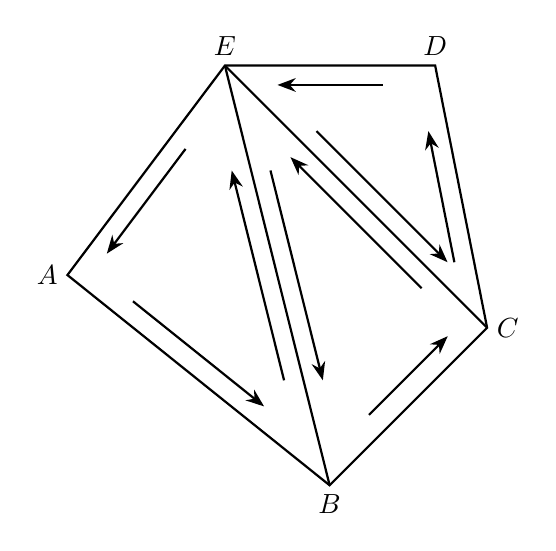
\begin{tikzpicture}
            \coordinate (A) at (0, 2.67);
            \coordinate (B) at (3.33, 0);
            \coordinate (C) at (5.33, 2);
            \coordinate (D) at (4.67, 5.33);
            \coordinate (E) at (2, 5.33);
            \draw[thick] (A) -- (B) -- (C) -- (D) -- (E) -- cycle;
            \draw[thick] (B) -- (E);
            \draw[thick] (C) -- (E);
            \halfarrow{[xshift=-7pt]B}{[xshift=-7pt]E}
            \halfarrow{[xshift=7pt]E}{[xshift=7pt]B}
            \halfarrow{[yshift=-11.2pt]E}{[yshift=-11.2pt]A}
            \halfarrow{[yshift=11.2pt]B}{[yshift=11.2pt]C}
            \halfarrow{[yshift=9.5pt]A}{[yshift=9.5pt]B}
            \halfarrow{[yshift=-9.4pt]C}{[yshift=-9.4pt]E}
            \halfarrow{[xshift=9.4pt]E}{[xshift=9.4pt]C}
            \halfarrow{[yshift=-7pt]D}{[yshift=-7pt]E}
            \halfarrow{[xshift=-7.14pt]C}{[xshift=-7.14pt]D}

            \node[anchor=east] at (A) {\(A\)};
            \node[anchor=north] at (B) {\(B\)};
            \node[anchor=west] at (C) {\(C\)};
            \node[anchor=south] at (D) {\(D\)};
            \node[anchor=south] at (E) {\(E\)};
        \end{tikzpicture}
        \caption{A closed polygonal chain internally triangulated, with orientations marked.}
        \label{fig:cauchyintegraltheoremoversimplyconnectedset_closedpolygonalchaintriangulation}
    \end{figure}Since \(P\) is a closed polygonal chain, we can triangulate the interior. For example, consider \autoref{fig:cauchyintegraltheoremoversimplyconnectedset_closedpolygonalchaintriangulation}. Then, \begin{align*}
        \int_{\partial ABCDE}f(z)\ddz & =\int_{\overrightarrow{AB}}f(z)\ddz+\int_{\overrightarrow{BC}}f(z)\ddz+\int_{\overrightarrow{CD}}f(z)\ddz+\int_{\overrightarrow{DE}}f(z)\ddz+\int_{\overrightarrow{EA}}f(z)\ddz \\
                                      & \quad+\int_{\overrightarrow{BE}}f(z)\ddz+\int_{\overrightarrow{EB}}f(z)\ddz+\int_{\overrightarrow{CE}}f(z)\ddz+\int_{\overrightarrow{EC}}f(z)\ddz                               \\
                                      & =\int_{\Delta{ABE}}f(z)\ddz+\int_{\Delta{BCE}}f(z)\ddz+\int_{\Delta{CDE}}f(z)\ddz.
    \end{align*} Thus, if the integral over every triangle in \(U\) vanishes, then \eqref{eq:cauchyintegraltheoremoversimplyconnectedset_statement} follows. Consider a triangle in \(U\) with boundary \(\Delta\). \begin{figure}
        \centering
        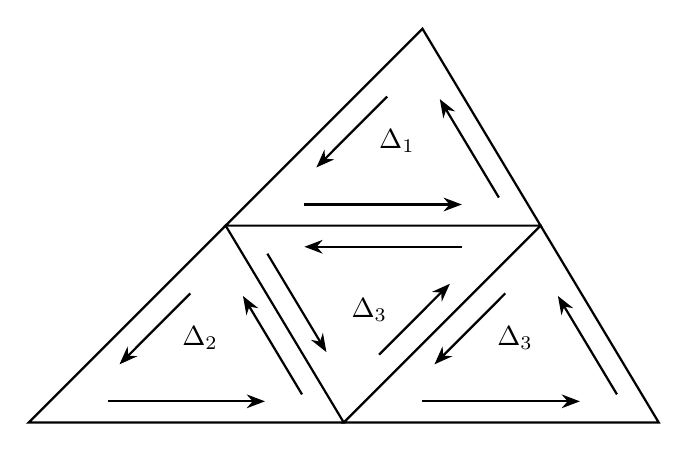
\begin{tikzpicture}
            \coordinate (A) at (0, 0);
            \coordinate (D) at (6.5, 2.5);
            \coordinate (F) at (2.5, 2.5);
            \coordinate (C) at (8, 0);
            \coordinate (B) at (5, 5);
            \coordinate (E) at (4, 0);

            \draw[thick] (A) -- (F) -- (E) -- cycle;
            \draw[thick] (B) -- (D) -- (F) -- cycle;
            \draw[thick] (C) -- (D) -- (E) -- cycle;

            \halfarrow{[yshift=-11.7pt]F}{[shift={(20pt, 8.2pt)}]A};
            \halfarrow{[yshift=-11.7pt]B}{[shift={(20pt, 8.2pt)}]F};
            \halfarrow{[yshift=-11.7pt]D}{[shift={(20pt, 8.2pt)}]E};
            \halfarrow{[yshift=11.7pt]E}{[shift={(-20pt, -8.2pt)}]D};

            \halfarrow{[shift={(-4.41pt, -7.64pt)}]E}{[shift={(-4.41pt, -7.64pt)}]F};
            \halfarrow{[shift={(-4.41pt, -7.64pt)}]D}{[shift={(-4.41pt, -7.64pt)}]B};
            \halfarrow{[shift={(-4.41pt, -7.64pt)}]C}{[shift={(-4.41pt, -7.64pt)}]D};
            \halfarrow{[shift={(4.41pt, 7.64pt)}]F}{[shift={(4.41pt, 7.64pt)}]E};

            \halfarrow{[yshift=7.64pt]A}{[yshift=7.64pt]E};
            \halfarrow{[yshift=7.64pt]E}{[yshift=7.64pt]C};
            \halfarrow{[yshift=7.64pt]F}{[yshift=7.64pt]D};
            \halfarrow{[yshift=-7.64pt]D}{[yshift=-7.64pt]F};

            \coordinate (AE) at ($(A)!0.5!(E)$);
            \coordinate (AF) at ($(A)!0.5!(F)$);
            \coordinate (FD) at ($(F)!0.5!(D)$);
            \coordinate (BF) at ($(B)!0.5!(F)$);
            \coordinate (EC) at ($(E)!0.5!(C)$);

            \path let
            \p1 = (FD),
            \p2 = (BF),
            \p3 = (AE),
            \p4 = (AF),
            \p5 = (EC)
            in
            node[shift={(5pt,-5pt)}] at (\x1, \y2) {\(\Delta_1\)}
            node[shift={(5pt,-5pt)}] at (\x3, \y4) {\(\Delta_2\)}
            node[shift={(5pt,-5pt)}] at (\x5, \y4) {\(\Delta_3\)}
            node[shift={(-5pt, 5pt)}] at (\x1, \y4) {\(\Delta_3\)};
        \end{tikzpicture}
        \caption{Quadrisection of the triangle bounded by \(\Delta\).}
        \label{fig:cauchyintegraltheoremoversimplyconnectedset_trianglequadrisection}
    \end{figure} Then define \(M\) to be \[M=\abs{\int_{\Delta}f(z)\ddz}.\]
    Quadrisect the triangle bounded by \(\Delta\) into four triangles with boundaries \(\Delta_1,\Delta_2,\Delta_3,\Delta_4\) as in \autoref{fig:cauchyintegraltheoremoversimplyconnectedset_trianglequadrisection}. Then one of \(\Delta_1\), \(\Delta_2\), \(\Delta_3,\), and \(\Delta_4\) (denote this to be \(\Delta^1\)) satisfy
    \[\int_{\Delta^1}f(z)\ddz\geq\frac{M}{4},\]
    and recursively, choose \begin{equation}
        \int_{\Delta^2}f(z)\ddz\geq\frac{M}{4^2},\ldots,\int_{\Delta^n}f(z)\ddz\geq\frac{M}{4^n}. \label{eq:cauchyintegraltheoremoversimplyconnectedset_trianglelowerbound}
    \end{equation} Let \(L\) denote the perimeter of \(\Delta\). Then, the perimeters of \(\Delta^1, \Delta^2,\ldots\) are \(\frac{L}{2},\frac{L}{2^2},\ldots\) respectively. As \(n\to\infty\), \(\Delta_n\) shrinks to a single point \(z_0\). Then, \(\forall n\in\mathbb{N}\), \(z_0\in\Delta^n\). 

    By the definition of holomorphy, \(\forall\varepsilon>0\), \(\exists\delta>0\) such that \(\forall z\in D\paren{z_0,\delta}\), \[\abs{\frac{f\paren{z}-f\paren{z_0}}{z-z_0}-f'\paren{z_0}}<\varepsilon,\]\[\abs{f\paren{z}-f\paren{z_0}-f'\paren{z_0}\paren{z-z_0}}<\varepsilon\abs{z-z_0}.\] and \(\exists N\in\mathbb{N}\) such that \(\forall n\in \mathbb{N}_{>N}\), \(\Delta^n\subset D\paren{z_0,\delta}\). By \autoref{thm:cauchyintegraltheorem}, since the functions \(1\) and \(z\) are both entire, \[\int_{\Delta^n}\ddz=0,\quad\int_{\Delta^n}z\ddz=0.\] Then 
    \begin{align*}
        \int_{\Delta^n}f(z)\ddz&=\int_{\Delta^n}f(z)\ddz-f\paren{z_0}\int_{\Delta^n}\ddz-f'\paren{z_0}\left(\int_{\Delta^n}z\ddz-z_0\int_{\Delta^n}\ddz\right)\\
        &=\int_{\Delta^n}\brackets{f(z)-f\paren{z_0}-f'\paren{z_0}\paren{z-z_0}}\ddz.
    \end{align*}
    Because the distance between any two points in the interior of a triangle is always less than its perimeter, using the triangle inequality for complex integrals, \[\int_{\Delta^n}\abs{f(z)}\abs{\ddz}\leq\varepsilon\int_{\Delta^n}\abs{z-z_0}\abs{\ddz}=\frac{\varepsilon L}{2^n}\int_{\Delta^n}\abs{\ddz}=\frac{\varepsilon L^2}{4^n}.\]
    Comparing the above equation with equation \eqref{eq:cauchyintegraltheoremoversimplyconnectedset_trianglelowerbound}, \[\frac{M}{4^n}<\frac{\varepsilon L}{4^n},\quad M<\varepsilon L.\] Since \(\Delta\) is rectifiable, \(L\) is finite, and letting \(\varepsilon\to0\), we find that \(M\to0\). For every triangle in \(U\), the integral vanishes, and equations \eqref{eq:cauchyintegraltheoremoversimplyconnectedset_chainvanishingstatement} and \eqref{eq:cauchyintegraltheoremoversimplyconnectedset_chaindefinition} follow.
\end{proof}
\begin{theorem}[Cauchy--Goursat Integral Theorem]\label{thm:cauchygoursattheorem}
    Let \(U\subset\mathbb{C}\) be an open region bounded with a piecewise \(C^1\) boundary \(\partial U\). Let \(f:U\to\mathbb{C}\) be a holomorphic function continuous on \(\overline{U}\). Then, \[\oint_{\partial U}f(\zeta)\ddzeta=0.\]
\end{theorem}
\begin{proof}
    \begin{figure}
        \centering
        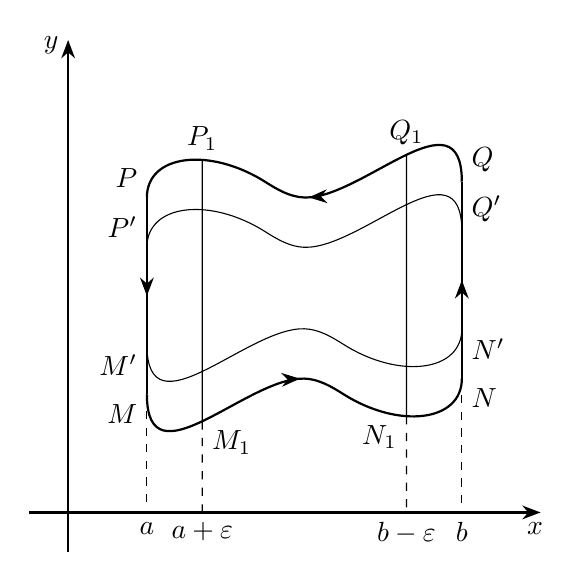
\begin{tikzpicture}[>=stealth,
            arrow style/.style={
                postaction={decorate},
                decoration={markings, mark=at position 0.5 with {\arrow[scale=1]{Stealth}}}
            }]
            \pgfmathsetmacro{\lengtheta}{18pt}
            \pgfmathsetmacro{\lengthepsilon}{20pt}

            \coordinate (M) at (1, 1.5);
            \coordinate (P) at (1, 4);
            \coordinate (Q) at (5, 4.2);
            \coordinate (N) at (5, 1.7);
            \coordinate (Mprime) at ([yshift=\lengtheta] M);
            \coordinate (Pprime) at ([yshift=-\lengtheta] P);
            \coordinate (Qprime) at ([yshift=-\lengtheta] Q);
            \coordinate (Nprime) at ([yshift=\lengtheta] N);
            
            \draw[-{Stealth}, thick] (-0.5, 0) -- (6, 0);
            \draw[-{Stealth}, thick] (0, -0.5) -- (0, 6);

            \draw[thick, arrow style] (P) -- (M);
            \draw[thick, arrow style, name path=curveQP] (Q) to[out angle=90, in angle=90, curve through = {([shift={(2, 0)}] P) ([shift={(1.5, 0.2)}] P)}] (P);
            \draw[thick, arrow style] (N) -- (Q);
            \draw[thick, arrow style, name path=curveMN] (M) to[out angle=270, in angle=270, curve through = {([shift={(-2, 0)}] N) ([shift={(-1.5, -0.2)}] N)}] (N);

            \path let \p1 = (P) in coordinate (P1x) at ({\x1 + \lengthepsilon}, 0);
            \path let \p1 = (Q) in coordinate (Q1x) at ({\x1 - \lengthepsilon}, 0);

            \path[name path=verticalleftmarker](P1x) -- (P1x |- 0, 6);
            \path[name path=verticalrightmarker](Q1x) -- (Q1x |- 0, 6);

            \path[name intersections={of=curveQP and verticalleftmarker, by=P1}];
            \path[name intersections={of=curveMN and verticalleftmarker, by=M1}];
            \draw[thin] (M1) -- (P1);

            \path[name intersections={of=curveQP and verticalrightmarker, by=Q1}];
            \path[name intersections={of=curveMN and verticalrightmarker, by=N1}];
            \draw[thin] (N1) -- (Q1);
            
            \draw[thin] (Mprime) to[out angle=270, in angle=270, curve through = {([shift={(-2, 0)}] Nprime) ([shift={(-1.5, -0.2)}] Nprime)}] (Nprime);
            \draw[thin] (Qprime) to[out angle=90, in angle=90, curve through = {([shift={(2, 0)}] Pprime) ([shift={(1.5, 0.2)}] Pprime)}] (Pprime);

            \draw[dashed] (M) -- (M |- 0, 0);
            \draw[dashed] (N) -- (N |- 0, 0);
            \draw[dashed] (M1) -- (P1x);
            \draw[dashed] (N1) -- (Q1x);

            \node[anchor=north east] at (M) {\(M\)};
            \node[anchor=south east] at (P) {\(P\)};
            \node[anchor=south west] at (Q) {\(Q\)};
            \node[anchor=north west] at (N) {\(N\)};
            \node[anchor=north east] at (Mprime) {\(M'\)};
            \node[anchor=south east] at (Pprime) {\(P'\)};
            \node[anchor=south west] at (Qprime) {\(Q'\)};
            \node[anchor=north west] at (Nprime) {\(N'\)};
            \node[anchor=north west] at (M1) {\(M_1\)};
            \node[anchor=south] at (P1) {\(P_1\)};
            \node[anchor=south] at (Q1) {\(Q_1\)};
            \node[anchor=north east] at (N1) {\(N_1\)};
            
            \node[anchor=north] at (M |- 0, 0) {\(a\)};
            \node[anchor=north] at (N |- 0, 0) {\(b\)};
            \node[anchor=north] at (P1x |- 0, 0) {\(a+\varepsilon\)};
            \node[anchor=north] at (Q1x |- 0, 0) {\(b-\varepsilon\)};

            \node[anchor=north, xshift=-2pt] at (6, 0) {\(x\)};
            \node[anchor=east, yshift=-2pt] at (0, 6) {\(y\)};
        \end{tikzpicture}
        \caption{}
        \label{fig:cauchygoursattheorem_simplifiedregion}
    \end{figure}
    Assume \(U\) has the shape of \autoref{fig:cauchygoursattheorem_simplifiedregion}.
\end{proof}
\begin{theorem}[Cauchy--Goursat Integral Formula]\label{thm:cauchygoursatformula}
    Let \(U\subset\mathbb{C}\) be an open region bounded with a piecewise \(C^1\) boundary \(\partial U \), and let \(f:U\to\mathbb{C}\) be a holomorphic function continuous on \(\overline{U}\). Then for all \(z\in U\),
    \begin{equation}
        f(z)=\frac{1}{2\pi i}\oint_{\partial U}\frac{f(\zeta)}{\zeta-z}\dd{\zeta}.\label{eq:cauchygoursatformula}
    \end{equation}
\end{theorem}
\end{document}